\title{ Fluid Flow Through Pipes \\
	SDI 374C Final Project }
\author{
       Joseph Voss \\
}
\date{\today}
\documentclass[12pt]{article}
\usepackage{listings}
\usepackage{courier}
\usepackage{graphicx}
\graphicspath{ {images/} }
\lstset{basicstyle=\footnotesize\ttfamily,breaklines=true}
\begin{document}
\maketitle

\section{Introduction and Purpose}
The topic I chose to research for this project was fluid flow. Originally I had intended to simulate the results
from a laboratory experiment I had completed earlier this semester by modeling the flow of fluid around a cylinder. 
However, I experienced a lot of difficulty simulating basic scenarios by solving the Navier Stokes equations, and 
instead decided to study the flow of fluid through a channel. While it may seem trivial, understanding this flow is 
essential to modern system design, and was the main focus of my fluid mechanics course in the latter half of the 
semester. The key aspects of interest are the pressure and velocity components as the flow travels, along with 
studying the viscous losses associated with the flow. 

To learn the basics of computational fluid mechanics I read several textbooks and online articles. However, the most 
useful resource by far was the 12 Steps to Navier Stokes online course published by the Lorena A. Barba research lab. 
Through a series of interactive ipython notebooks they model several types of one dimensional and two dimensional 
flows, before eventually building up to a basic solution of the Navier Stokes equations. This resource showed me a 
relatively simple was to model fluid flow, and provided the equations necessary along with a rough outline of the 
different steps required to solve them.

\section{Algorithm to be Parallelized}
To solve this problem the two dimensional Navier Stokes equations were used in addition to the Possion Pressure 
equation. These are all second order differential equations and will have to be approximated discretely. The original 
equations are depicted below, and offer a comprehensive description of Newtonian viscous flow. Additionally, if the 
flow is assumed to be incompressible, (an assumption which is valid for flows with a Mach number slower than 0.3) then 
the Possion Pressure equation can be used as a continuity constraint. Together these three equitation's allow for the 
pressure along with the  horizontal and vertical velocity at each point to be known.

Navier Stokes X-Momentum
$$\frac{\partial u}{\partial t}+u\frac{\partial u}{\partial x}+v\frac{\partial u}{\partial y}=-\frac{1}{\rho}\frac{\partial p}{\partial x}+\nu\left(\frac{\partial^2 u}{\partial x^2}+\frac{\partial^2 u}{\partial y^2}\right)$$

Navier Stokes Y-Momentum
$$\frac{\partial v}{\partial t}+u\frac{\partial v}{\partial x}+v\frac{\partial v}{\partial y}=-\frac{1}{\rho}\frac{\partial p}{\partial y}+\nu\left(\frac{\partial^2 v}{\partial x^2}+\frac{\partial^2 v}{\partial y^2}\right)$$

Possion Pressure Equation
$$\frac{\partial^2 p}{\partial x^2}+\frac{\partial^2 p}{\partial y^2}=-\rho\left(\frac{\partial u}{\partial x}\frac{\partial u}{\partial x}+2\frac{\partial u}{\partial y}\frac{\partial v}{\partial x}+\frac{\partial v}{\partial y}\frac{\partial v}{\partial y}\right)
$$

Due to viscous effects fluid traveling in a channel or pipe develops a head loss, and need some force to drive the 
flow. Therefore a constant force was added to the X-Momentum equation. Once these equations are discretized they can 
be rearranged to solve for the next time step for the horizontal and vertical velocity. This can be done because the 
momentum equations have a component of velocity that is differentiated by time. However, in the pressure equation the 
pressure terms are only differentiated by the x and y dimensions. Therefore, the pressure equation needs to be solved 
by successive iterations, while the momentum equations can be solved in a single time step.

%Note that these equations need to have boundary conditions to be solved. 

\section{How that Parallelization was achieved, design goals}

The continuous flow region was divided into a grid composed of several uniform cells. Each of these cells have their 
own horizontal and vertical velocity components and along with a pressure value. These cells can be solved 
independently within each time-step, and are thereby suitable for parallelization using MPI. The solved values for 
each cell are distributed among the different processors used. To solve each cell the values of it's neighbors need 
to be known, so there has to be some communication at the end of each time step. These communicated values are then 
used in the discritized equations to solve for the values of each cell at the next time step. This continues for the 
specified amount of time and for each cell in the grid. The cells are divided up linearly and assigned to a processor. 
If the number of cells are not evenly divisible, then the remaining cells are added to separate processors one at a 
time. By doing so the most unequal workload would be one additional cell on some processors. If each processor has 
several hundred cells already, this imbalance is negligible.

The algorithm stated in the previous section was broken into two main stages; the pressure solving and the velocity 
solving. The pressure solution for each cell needs to be done in pseudo-time, with communication between processors at 
the end of each pseudo-time step. However, only the previous pressure components actually change with each pseudo-time 
step. The other components of the pressure equation are all due to the velocity, which doesn't change during the 
pseudo-time steps. Therefore the pressure equation can be broken into two parts. The velocity component's contribution 
to the pressure is solved at the beginning of each full time step, while the pressure components are modified within 
the pseudo-time loop. At the end of each pseudo-time step these two pieces are added together to find the pressure for 
the current cell. By moving the constant velocity components out of the pseudo-time loop the total computation for 
each pseudo-time step is cut in half. Once all of a processor's cells have been solved for then an all gather vector 
communication is performed. The all gather collects each of the data from the processors local cells, then broadcasts 
it to all of the other processors and stores in their individual global arrays. This solves the issue of distributed 
data for each cell, allowing them to know the values of their neighbors for their individual calculations. An all 
gather vector was needed here instead of a regular all gather because of the potential unequal loading of the 
processors. The number of cells on each processor is found initially and broadcast to every processor so the 
variable length communication can take place.

Once the pressure for each cell is found the velocity components can be found in a similar fashion. The velocity 
components only require one time step to find a solution however, instead of iterating over pseudo-time steps in 
addition to the actual time steps. Using the pressure and velocity found for the previous time step the X and Y 
components of velocity for the current step can be found. This is then stored along with the previously found pressure 
for this time step in an multi-dimensional array of structs. Once this is done for each cell on the processor another 
vector all gather is performed, distributing the data from each cell to an array in each processor. Once this is done 
the time step is incremented, and the pressure and velocity data for each cell is found again. This continues until 
the last time step is reached, after which the data is written out sequentially to an HDF5 file for post-processing 
visualization. A pseudo-code representation of this parallelization is shown below.

\begin{lstlisting}
while counter < numberTimeSteps
	//Make initial pressure array and 
	//Find velocity component of pressure
	for i in numCells
		solvedPressure[0][i] = solvedData[counter-1][i].p
		velocityComponent[i] = presVelComponent(xLocation,yLocation)
	
	//Find pressure
	while subCounter < numberPseudoTimeSteps
		for i in numCells
			localPresData[i] = pressSolve(xLocation,yLocation)

		MPI_Allgatherv(localPresData, solvedPrePresData[subCounter])

		subCounter += 1;

	//Find velocity and store data
	for i in numCells
		localData[i].u = xMomentumSolve(xLocation, yLocation)
		localData[i].v = yMomentumSolve(xLocation, yLocation)
		localData[i].p = solvedPressure[numberPseudoTimeSteps-1][startingLocation+i]

	MPI_Allgatherv(localVelData,  solvedVelData[counter][0])

	subCounter = 1
	counter += 1
\end{lstlisting}

\section{Timing Results and Trace}
The program was run for a 300x300 size grid with 500 time steps and 300 pseudo-time steps. The timing results for this 
large-scale run can be seen in Figure 1. As one can see, the run time actually increases with the number of 
cores initially. The reason behind this can be seen in the trace diagram for a small-scale version of this program in 
Figure 2. One can 
see the large blocks of MPI communication which fills up most of the diagram. The tiny slivers of brown green in 
between them are where the actual calculations are being performed. Therefore the timing behavior observed makes 
intuitive sense. For large work loads the performance is increased as the number of processors increase, to a certain 
extent. Once the workload on each processor is light enough the communication between the processors becomes a much 
more limiting factor than the calculations itself. After this point, additional processors will do nothing fill the 
network with more communications and make the program more and more reliant on slow communications to do the same 
amount of work. This explains why the performance gain per processor isn't a linear or even asymptotic curve, but 
rather can actually increase the run time of the program. However, the run time then drastically decreases as 
more processors are added, which is not the expected behavior at all and I don't understand. The efficiency is very 
low though, seeing as how with 80 processors the program runs slower than 5 processors.

\begin{figure}[ht]
\centering
\caption{ Timing results, Number of Processors vs. Runtime (s)}
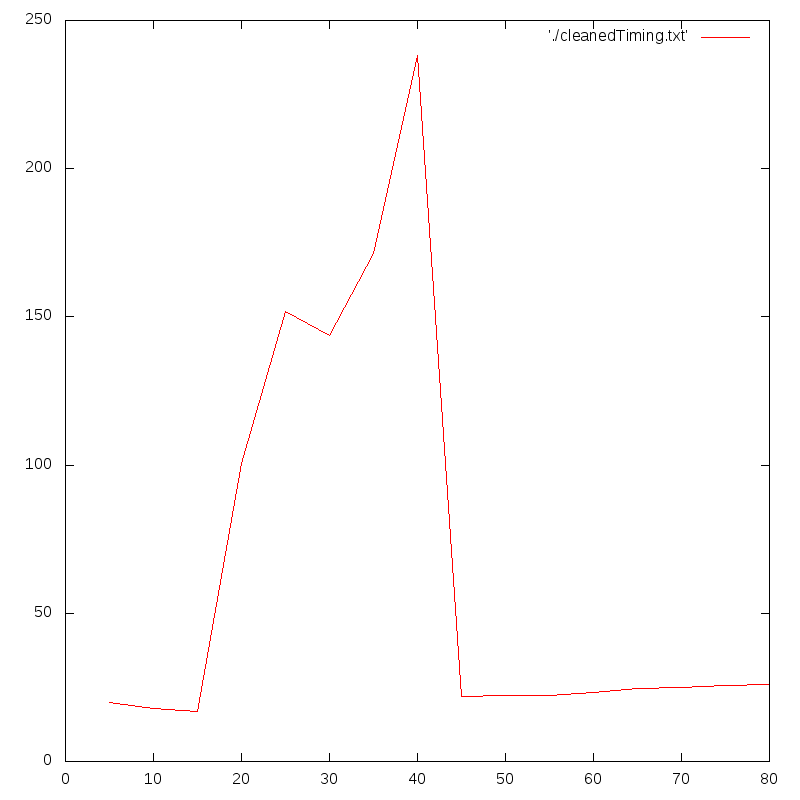
\includegraphics[width=0.75\textwidth]{output.png}
\end{figure}
\begin{figure}[ht]
\centering
\caption{TAU trace of the program}
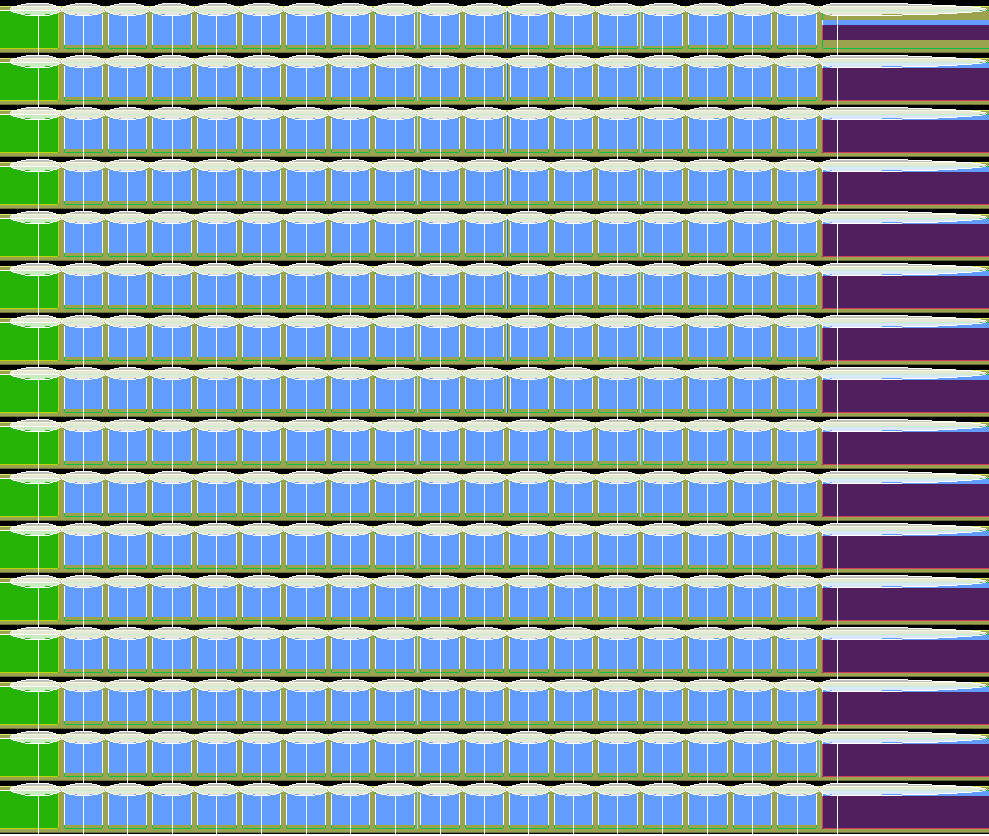
\includegraphics[width=0.75\textwidth]{trace.png}
\end{figure}


In Figure 3 one can see the solved image of flow for laminar flow through a channel. The constant color background means 
that the pressure is constant everywhere, and the viscous effects due to the walls clearly reduce the energy of the 
flow. Because the velocity gradient isn't a parabola this means that the flow is still developing, and viscous effects 
will become more dominant as time progresses. All of these observations coincide exactly with the ideal and 
experimental behavior of two dimensional flow through a pipe, thus proving that the model was successful in modeling 
flow under these conditions.
\begin{figure}[h]
\centering
\caption{The solved velocity and pressure data}
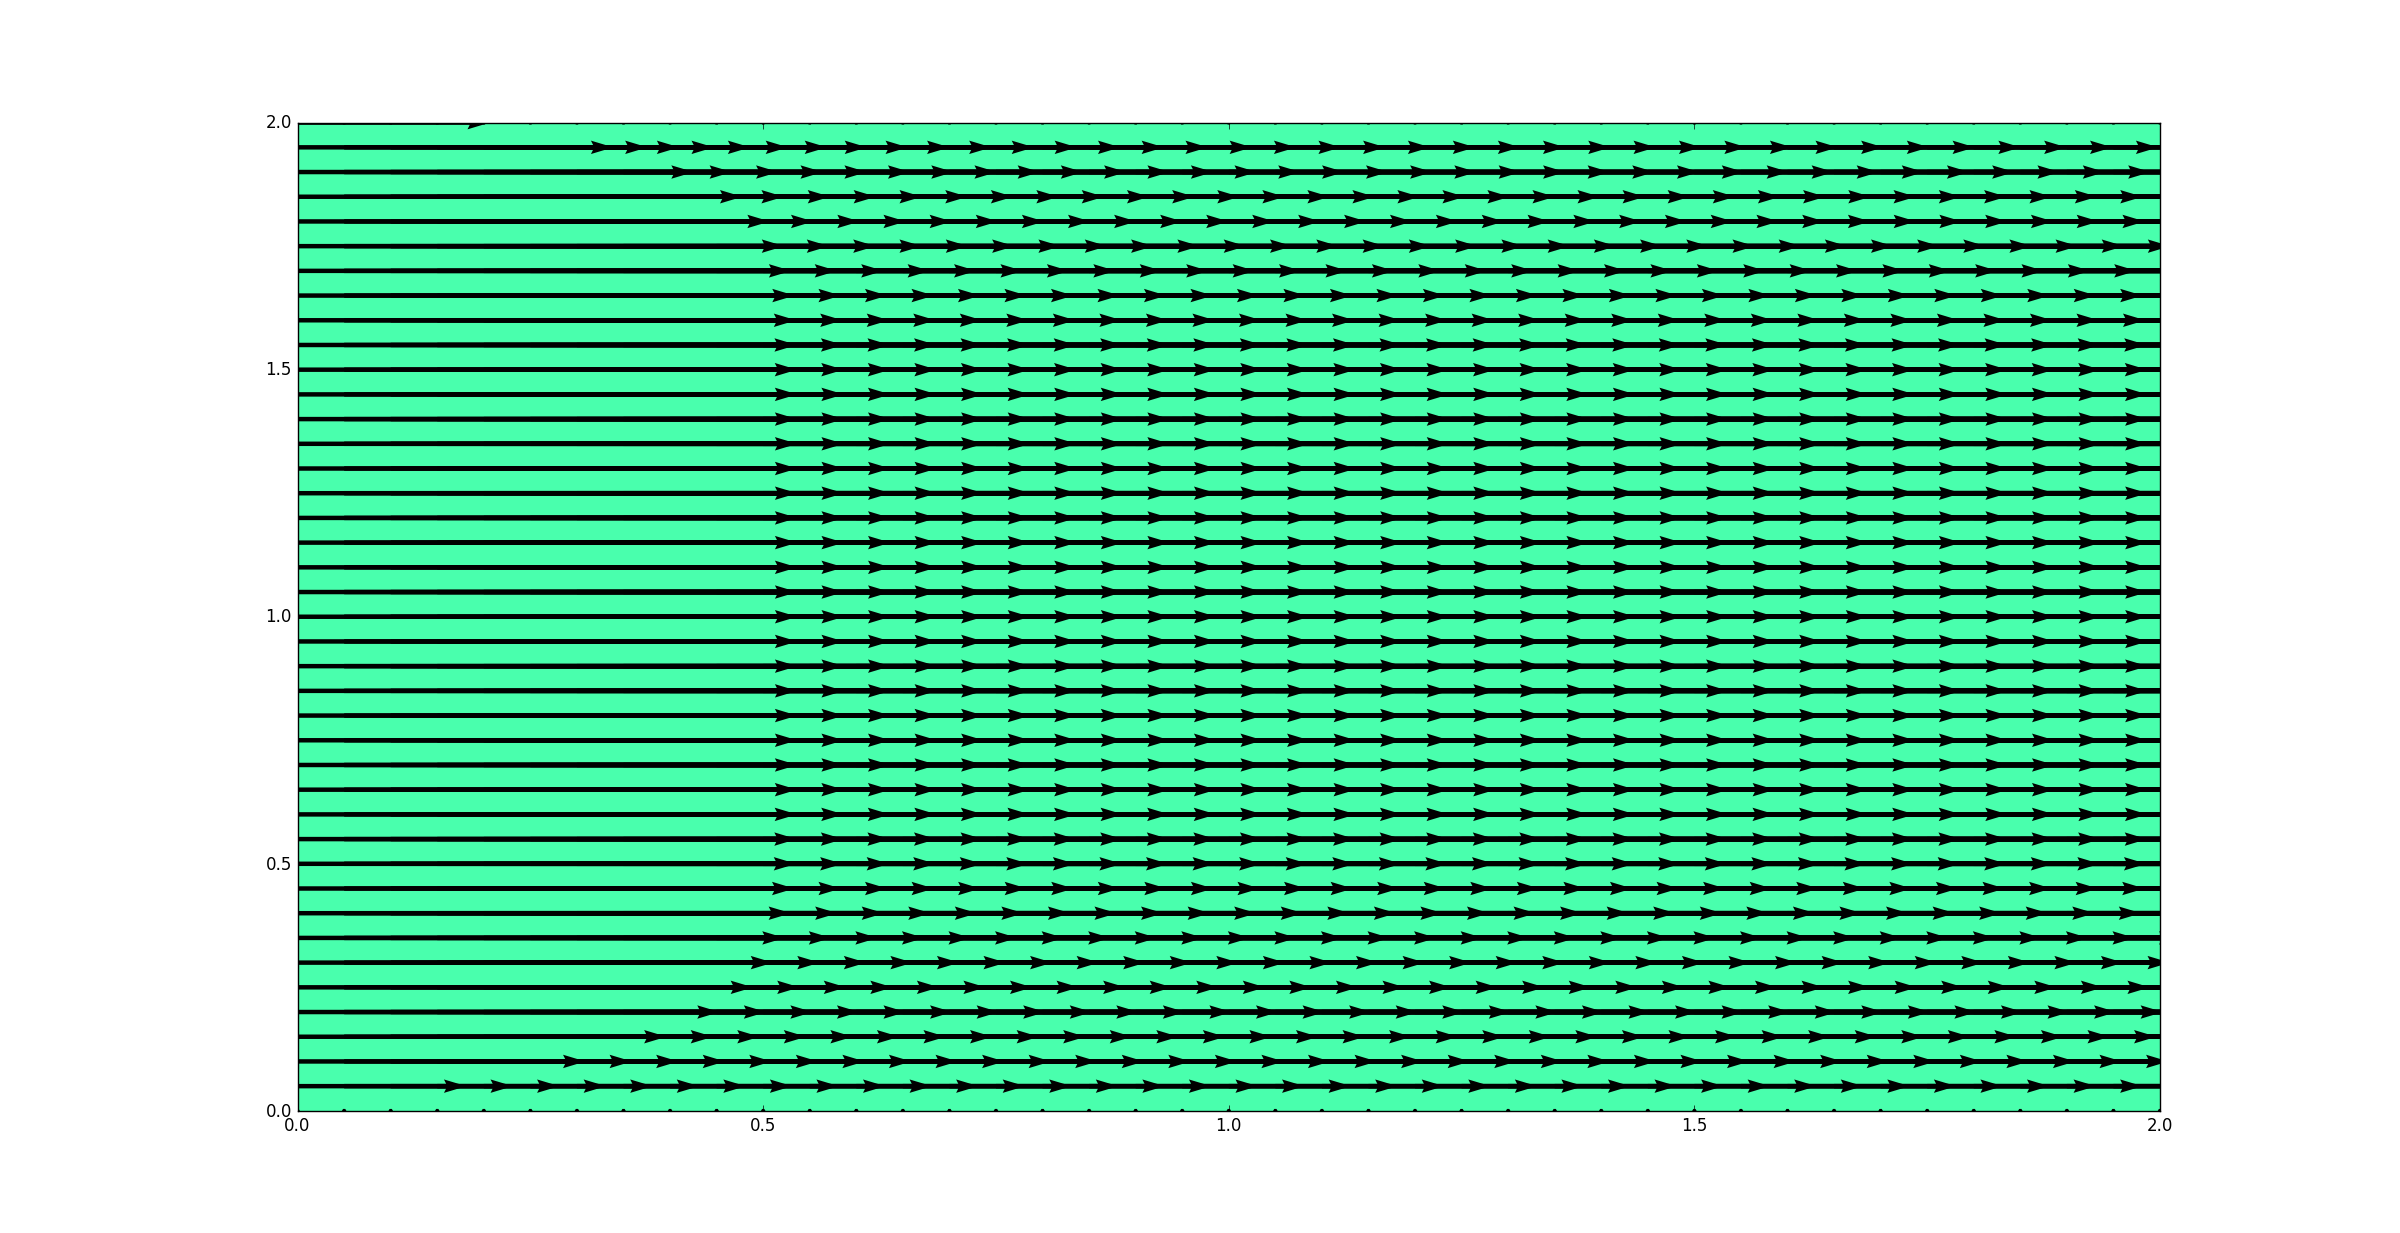
\includegraphics[width=0.75\textwidth]{solvedFlow2.png}
\end{figure}

\end{document}
